\PassOptionsToPackage{table,x11names}{xcolor}
\documentclass[leqno, 10pt, envcountsect]{beamer}

%------------------------------+
% Silence compilation warnings |
%------------------------------+
% Silence biblatex and caption warning when used with beamer
\usepackage{silence}
\WarningFilter{biblatex}{Patching footnotes failed}
\WarningFilter{caption}{Forced redefinition of}

%---------------------------------------+
% Source code, programming and patching |
%---------------------------------------+
\usepackage{embedfile}                 % Embed latex source code
% \embedfile{clase_ml.tex}
\usepackage{etoolbox}                  % Toolbox of programming tools
\usepackage{xpatch}                    % Extension of etoolbox patching commands

%--------------------------------------+
% Language, hyphenation, encoding, etc |
%--------------------------------------+
% Babel package
\usepackage[english,spanish,es-noindentfirst,es-nosectiondot,es-nolists,
es-noshorthands,es-lcroman,es-tabla]{babel}

\usepackage{lmodern}             % Use Latin Modern fonts
\usefonttheme[onlymath]{serif}   % Computer modern fonts in math
\usefonttheme{professionalfonts} % Prevent undesired replacements by beamer
\usepackage[T1]{fontenc}         % Better output when a diacritic/accent is used
\usepackage[utf8]{inputenc}      % Allows to input accented characters
\usepackage{textcomp}            % Avoid conflicts with siunitx and microtype
\usepackage{microtype}           % Improves justification and typography

% Translator package (loaded by beamer)
\uselanguage{spanish}
\languagepath{spanish}
\deftranslation[to=spanish]{Notation}{Notación}
\deftranslation[to=spanish]{Remark}{Observación}
\deftranslation[to=spanish]{Problem}{Enunciado}


\usepackage{changepage}

%-------------------------------------+
% Beamer style: theme, frames, titles |
%-------------------------------------+
% Use the default theme (alternative define another one like this:)
% \usetheme{Madrid}

% Frames (empty navigation bar and add roman number title when a frame is split)
\beamertemplatenavigationsymbolsempty
\setbeamertemplate{frametitle continuation}[from second][
  \insertcontinuationcountroman]

% Reduce margins (i.e increase textwidth)
\setbeamersize{text margin left=0.35cm,text margin right=0.35cm}

% Define color
\definecolor{jampp_color}{RGB}{54,53,91}

% Set frametitle, title and date color
\setbeamercolor*{title}{fg=jampp_color}
\setbeamercolor*{frametitle}{fg=black}
\setbeamerfont{frametitle}{size=\normalsize, series=\bfseries}
\setbeamertemplate{frametitle}{\hspace{-0.1cm}
  \expandafter\MakeUppercase\expandafter\insertframetitle
}

% Insert Page number in footline
\defbeamertemplate*{footline}{example theme}
{\begin{beamercolorbox}[wd=\paperwidth, dp=2.5ex]{}
  \hfill\textcolor{jampp_color}{\scriptsize{\insertframenumber}}\hspace{0.4cm}
\end{beamercolorbox}
}

% Insert rule and logo in headline (load tikz package for this)
% To make this work with multiline frametitle see:
% https://tex.stackexchange.com/a/386733/9953
\usepackage{tikz}
\usetikzlibrary{arrows,intersections,calc,decorations.pathreplacing,
decorations.markings}
\addtobeamertemplate{frametitle}{}{%
\begin{tikzpicture}[remember picture,overlay]
\node[anchor=south west, yshift=-2pt, xshift=1pt] at (current page.south west)
{
\includegraphics[scale=0.022]{logo_mutt.png}};
\draw[jampp_color] ([yshift=-0.65cm, xshift=0.25cm]current page.north west)
  -- ([yshift=-0.65cm, xshift=\paperwidth - 0.25cm]current page.north west);
\end{tikzpicture}}

% Comment or uncomment to see notes
% \setbeameroption{show notes}
% Display notes with item option as an itemize environment (instead of an
% enumerate one)
\AtBeginNote{%
  \let\enumerate\itemize%
  \let\endenumerate\enditemize%
}
% \setbeameroption{show notes on second screen=right}

%-------------------------------+
% Math symbols and environments |
%-------------------------------+
\numberwithin{equation}{section}
\usepackage{amssymb}    % Defines most math symbols (such as \mathbb)
\usepackage{mathtools}  % Extension and bug fixes for amsmath package
\usepackage{mathrsfs}   % Math script like font
\usepackage{breqn}      % Automatic line breaking of math expressions
\renewcommand*{\intlimits}{\displaylimits}  % Fix breqn clash with intlimits

%------------------------------------+
% Definition of theorem environments |
%------------------------------------+
\setbeamertemplate{theorems}[numbered]

% Define numbered and unnumbered theorem environments
\newtheorem*{theorem*}{\translate{Theorem}}
\newtheorem{proposition}[theorem]{\translate{Proposition}}
\newtheorem*{proposition*}{\translate{Proposition}}
\newtheorem*{lemma*}{\translate{Lemma}}
\newtheorem*{corollary*}{\translate{Corollary}}

\theoremstyle{definition}
\newtheorem*{definition*}{\translate{Definition}}
\undef{\example}
\newtheorem{example}[theorem]{\translate{Example}}
\newtheorem*{example*}{\translate{Example}}
\newtheorem{exercise}[theorem]{\translate{Exercise}}
\newtheorem*{exercise*}{\translate{Exercise}}
\newtheorem*{problem*}{\translate{Problem}}
\newtheorem*{solution*}{\translate{Solution}}

\setbeamercolor*{block title example}{fg=white,bg=structure.fg!75!black}
\setbeamerfont{block title example}{shape=\itshape}
\theoremstyle{example}
\newtheorem{remark}[theorem]{\translate{Remark}}
\newtheorem*{remark*}{\translate{Remark}}
\newtheorem*{notation*}{\translate{Notation}}

% Remove dot from proof environment
\makeatletter
  \AtBeginEnvironment{proof}{\let\@addpunct\@gobble}
\makeatother

%---------------------+
% Floats and captions |
%---------------------+
% Beamer loads graphicx package by default and centers floats in figure and
% table environments
\graphicspath{{figures/}{tables/}}

% We use load compatibility false to allow caption setup to work with beamer and
% set caption skip since we do not use floatrow which resets it
\usepackage[skip=\dimexpr\abovecaptionskip-2pt,compatibility=false]{caption}
\setbeamerfont{caption}{size=\small}
\setbeamercolor*{caption name}{fg=structure.fg!75!black}
\captionsetup*[figure]{format=plain,justification=centerlast,labelsep=quad}
\captionsetup*[table]{justification=centering,labelsep=newline}
\setbeamertemplate{caption}[numbered]
\numberwithin{figure}{section}
\numberwithin{table}{section}

% Use subcaption for subfigures (to work properly with hyperref)
\usepackage{subcaption}
\captionsetup*[subfigure]{font=footnotesize,subrefformat=simple,
  labelformat=simple}
\renewcommand*{\thesubfigure}{(\alph{subfigure})}

% FIXME: floatrow doesn't work without a placement option; is it needed?
% \usepackage[captionskip=5pt]{floatrow}  % Further modifications of float layout
% \floatsetup[table]{style=Plaintop,font=small,footnoterule=none,footskip=2.5pt}

% \usepackage{longtable}        % Allows to break tables through pages
% \floatsetup[longtable]{margins=centering,LTcapwidth=table}

%------------------------------------------------------+
% Miscellaneous packages: lists, listings, lipsum, etc |
%------------------------------------------------------+
% Lists symbols and colors
\useinnertheme{circles}

% Itemize
\newcommand*\smallcircled[1]{\tikz{
  \node[shape=circle,draw,inner sep=1.6pt] (char) {#1};}}
\setbeamertemplate{itemize item}{\large{$\bullet$}}
\setbeamertemplate{itemize subitem}{\smallcircled{}}
\setbeamertemplate{itemize subsubitem}{--}
\setbeamercolor*{itemize item}{fg=jampp_color}
\setbeamercolor*{itemize subitem}{fg=jampp_color}
\setbeamercolor*{itemize subsubitem}{fg=jampp_color}
\setlength{\leftmargini}{0.4cm}

% Enumerate
% Note: For a list of steps give the optional argument [Step 1.] to enumerate
% To use projected enumeration items comment the following line
\setbeamertemplate{enumerate items}[default]
\setbeamercolor*{item projected}{bg=jampp_color, fg=white}
\setbeamercolor*{enumerate item}{fg=jampp_color}
\setbeamercolor*{enumerate subitem}{fg=jampp_color}
\setbeamercolor*{enumerate subsubitem}{fg=jampp_color}
\renewcommand{\insertsubenumlabel}{\alph{enumii}}
\renewcommand{\insertsubsubenumlabel}{\roman{enumiii}}

% Increase item separation a bit
\let\olditem\item
\renewcommand{\item}{%
\olditem\vspace{1pt}}

% Temporary counter to store enumerate value
\newcounter{enumtemp}

% Code insertion (note: requires pygment python library and shell pdflatex flag)
\usepackage{minted}
% Define bg_color and frame border (using tcolorbox)
\definecolor{notebook_bg}{RGB}{247,247,247}
\definecolor{notebook_border}{RGB}{207,207,207}
\usepackage{tcolorbox}
\BeforeBeginEnvironment{minted}{\begin{tcolorbox}[colframe=notebook_border,
colback=notebook_bg, boxrule=0.4pt, left=0pt, top=0pt, bottom=0pt]}%
\AfterEndEnvironment{minted}{\end{tcolorbox}}%
% Set minted style
\setminted{style=default, fontsize=\scriptsize, autogobble}

% \usepackage{lipsum}    % Dummy text generator

\usepackage[normalem]{ulem} % strikethrough

%--------------------------+
% References and footnotes |
%--------------------------+
% Language sensitive quotation facilities
\usepackage[style=american]{csquotes}

\usepackage[style=authoryear-comp,backref=true,hyperref=false,
backend=biber]{biblatex}
\usepackage{mybibformat} % Modifications to authoryear-comp style and hyperlinks
% Beamer specific font and icon modifications
\setbeamercolor*{bibliography entry author}{fg=black}
\setbeamercolor*{bibliography entry note}{fg=black}
% \setbeamertemplate{bibliography item}{}
% Name of bibfile
\addbibresource{clase_ml.bib}


% Reduce footnote rule length
\renewcommand*{\footnoterule}{\vspace*{0.2cm}\hrule width 2.5cm\vspace*{0.2cm}}

%--------------------------------------------+
% Hyperlinks, bookmarks and cross-references |
%--------------------------------------------+
% Beamer hyperlink buttons
\setbeamercolor{button}{bg=structure.fg!75!black,fg=white}
\setbeamerfont{button}{size=\scriptsize}

% Hyperref setup
\hypersetup{colorlinks=true, allcolors=structure.fg!92!black,
pdfcreator={Vim LaTeX}, pdfsubject={python, linux},
pdftitle={Introducción Práctica a Machine Learning con Python},
pdfauthor={Mutt Data},
pdfkeywords={python, machine learning}
}

% Add anchor for equations, figures and tables
\makeatletter
\newcounter{phantomtarget}
\renewcommand*{\thephantomtarget}{phantom.\the\value{phantomtarget}}
\newcommand*{\phantomtarget}{%
  \stepcounter{phantomtarget}%
  \hypertarget{\thephantomtarget}{}%
  \edef\@currentHref{\thephantomtarget}%
}
\makeatother
% We use \appto to account for allowframbreaks
\appto{\equation}{\phantomtarget}
\appto{\figure}{\phantomtarget}
\appto{\table}{\phantomtarget}
\appto{\proposition}{\phantomtarget}
\appto{\corollary}{\phantomtarget}
\appto{\definition}{\phantomtarget}
\appto{\exercise}{\phantomtarget}
\appto{\remark}{\phantomtarget}
\appto{\problem}{\phantomtarget}
\appto{\solution}{\phantomtarget}
% For some theorems we use \AtBeginEnvironment due to the optional name argument
\AtBeginEnvironment{theorem}{\phantomtarget}
\AtBeginEnvironment{example}{\phantomtarget}
\AtBeginEnvironment{lemma}{\phantomtarget}
% \AtBeginEnvironment{subfigure}{\phantomtarget}

% Hyperlink parentheses and create cleveref-like command
\renewcommand*{\eqref}[1]{\hyperref[#1]{(\ref*{#1})}}
\newcommand{\crefnostar}[1]{\hyperref[#1]{\ref*{#1}}}
\newcommand{\crefstar}[1]{\ref*{#1}}      % No hyperlink (useful for proof env.)
\makeatletter
\newcommand{\cref}{\@ifstar{\crefstar}{\crefnostar}}
\makeatother

% Bookmarks for each frame
% TODO: Use short section names
\usepackage[open, openlevel=1]{bookmark}
\makeatletter
\apptocmd{\beamer@@frametitle}{\only<1>{%
  \bookmark[page=\the\c@page,level=3]{#1 \expandafter%
    \ifnum\insertcontinuationcount>1%
      \relax\insertcontinuationcountroman%
    \fi}%
  }}%
\makeatother

%------------------------+
% Title and TOC settings |
%------------------------+
% Reduce date font and change title and subtitle color
\setbeamerfont{title}{shape=\bfseries, size=\Large}
\setbeamerfont{subtitle}{series=\mdseries}
\setbeamerfont{date}{size=\scriptsize}
\setbeamercolor{title}{fg=jampp_color}

% Use uppercase for title and subtitle
\makeatletter
\setbeamertemplate{title page}{%
  \vbox{}
  \vfill
  \begingroup
    \vspace{1cm}  % for centering
    \centering
    \begin{beamercolorbox}[sep=8pt,center]{title}
    \usebeamerfont{title}\MakeUppercase{\inserttitle}\par%
    \ifx\insertsubtitle\@empty%
    \else%
      \vskip0.25em%
      {\usebeamerfont{subtitle}\usebeamercolor[fg]{subtitle}\MakeUppercase{\insertsubtitle}\par}%
    \fi%
  \end{beamercolorbox}%
  \vskip1em\par
  \begin{beamercolorbox}[sep=8pt,center]{author}
    \usebeamerfont{author}\insertauthor
  \end{beamercolorbox}
  \begin{beamercolorbox}[sep=8pt,center]{institute}
    \usebeamerfont{institute}\insertinstitute
  \end{beamercolorbox}
  \begin{beamercolorbox}[sep=8pt,center]{date}
    \usebeamerfont{date}\insertdate
  \end{beamercolorbox}\vskip0.5em
  {\usebeamercolor[fg]{titlegraphic}\inserttitlegraphic\par}
  \endgroup
  \vfill
}
\makeatother

% Increase separation between top of the slide and title
\makeatletter
\expandafter\patchcmd\csname beamer@@tmpl@title page\endcsname%
  {\vfill}{\vspace*{0.3cm}}{}{}
\makeatother

% Actually define maketitle
\title[Intro ML Python]{Introducción Práctica a Machine Learning con Python y
Spark}
\subtitle{Especialización en Ciencia de Datos - ITBA}
\author[]{Workshop de Big Data}
\institute[]{8 de Abril de 2020}
\date[]{
\includegraphics[scale=0.07]{logo_mutt.png}}

% Add agenda toc frame at the beginning of each section and anchor for proper
% hyperlinking
\AtBeginSection[]{
  \phantomtarget
  \begin{frame}[fragile=singleslide]
    \frametitle{Agenda}
    \tableofcontents[currentsection]
  \end{frame}
}
% Increase TOC number size
\setbeamerfont{section number projected}{size=\footnotesize}
% Change toc bullets to circles and use black color
\newcommand*\circled[1]{\tikz[baseline=(char.base)]{
  \node[shape=circle,draw=jampp_color,inner sep=2pt,
  line width=0.6pt, text=black] (char) {#1};}}
\setbeamertemplate{section in
toc}{\circled{\small{\inserttocsectionnumber}}~%
\bfseries{\inserttocsection}}

%---------------------------------------------------+
% (Re)Definition of new commands and math operators |
%---------------------------------------------------+
% Numbers
\DeclareMathOperator{\N}{\mathbb{N}}
\DeclareMathOperator{\Z}{\mathbb{Z}}
\DeclareMathOperator{\Q}{\mathbb{Q}}
\DeclareMathOperator{\R}{\mathbb{R}}
% Probability
\DeclareMathOperator{\E}{\mathbb{E}}
\DeclareMathOperator{\var}{\mathrm{Var}}
\DeclareMathOperator{\cov}{\mathrm{Cov}}
% Delimiters
\DeclarePairedDelimiter{\abs}{\lvert}{\rvert}
\DeclarePairedDelimiter{\norm}{\lvert\lvert}{\rvert\rvert}
% Miscellaneous
\renewcommand{\d}{\ensuremath{\operatorname{d}\!}}  % Differential
\renewcommand{\L}{\ensuremath{\operatorname{\mathcal{L}}}}  % Lagrangian


\begin{document}

\frame[plain]{\titlepage}

\section{Un breve repaso del (necesario) contexto teórico}
\label{sec:un_poco_de_contexto_teorico}

\begin{frame}[fragile=singleslide]
  \frametitle{Machine Learning o Aprendizaje Automático}
  \begin{itemize}
    \item Subcampo o técnica de la \textbf{minería de datos} (o \textit{data mining})
      \begin{itemize}
        \item Proceso de negocios que explora grandes volúmenes de datos con el
          fin de descubrir \textbf{patrones y reglas significativas}.
        \begin{itemize}
          \item Ejemplos: encontrar características de clientes que se dan de
            baja; productos que se venden previos a catástrofe natural, etc.
        \end{itemize}
      \end{itemize}

    \item Definición clásica [\textcite{mitchell97}]:\\
    \begin{quote}
      \enquote{Un \textbf{programa de computadora} se dice que aprende de la
      \textbf{experiencia} $E$ con respecto a una clase de \textbf{tareas} $T$ y
      \textbf{medida de performance} $P$, si su performance en las tareas en
      $T$, medidas con $P$, mejoran con la experiencia $E$.}
    \end{quote}
    \begin{itemize}
      \item Donde:
        \begin{itemize}
      \item Programa de computadora $\simeq$ modelo estadistico
      \item Experiencia $E$ $\simeq$ datos
      \item Ejemplo: predecir la altura de un niño a 6 meses vista ($T$)
      \end{itemize}
    \end{itemize}
  \end{itemize}
\end{frame}
\begin{frame}[fragile=singleslide]
  \frametitle{Tipos o familias de aprendizaje}
  \begin{itemize}
    \item Existen tres grandes familias de algoritmos de aprendizaje automático
      \begin{enumerate}
        \item \textbf{Supervisado}: los datos son \textit{instancias
          etiquetadas}, pares de objetos dados por observaciones y respuestas
          asociadas
          \begin{itemize}
            \item Objetivo: generar una función que relacione los datos de
              entrada con los de salida y pueda ser utilizada con datos
              desconocidos
          \item Ejemplos/Aplicaciones: filtros de Spam, tasa de conversión en
            marketing online
          \end{itemize}
        \item \textbf{No Supervisado}: los datos son observaciones sin
          respuestas asociadas
          \begin{itemize}
            \item Objetivo: comprender las relaciones subyacentes entre las
              distintas observaciones
          \item Ejemplos/Aplicaciones: clustering
          \end{itemize}
        \item \textbf{Por Refuerzos}: los datos definen un entorno, un conjunto
          de estados y acciones y funciones de pago (premios/castigos)
        \begin{itemize}
          \item Objetivo: encontrar una regla o política de acción que maximice
            el beneficio esperado
          \item Ejemplos/Aplicaciones: agentes económicos, Pacman.
        \end{itemize}
      \end{enumerate}
  \end{itemize}
  \begin{center}
    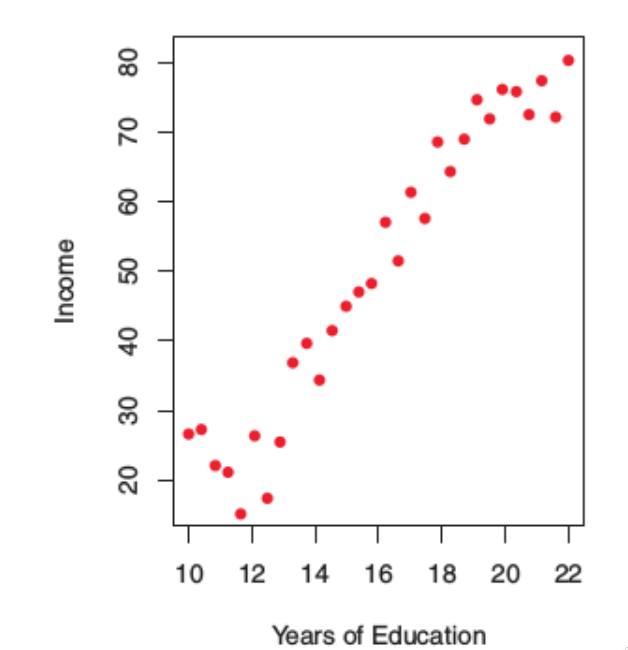
\includegraphics[scale=0.16]{supervised.png}
    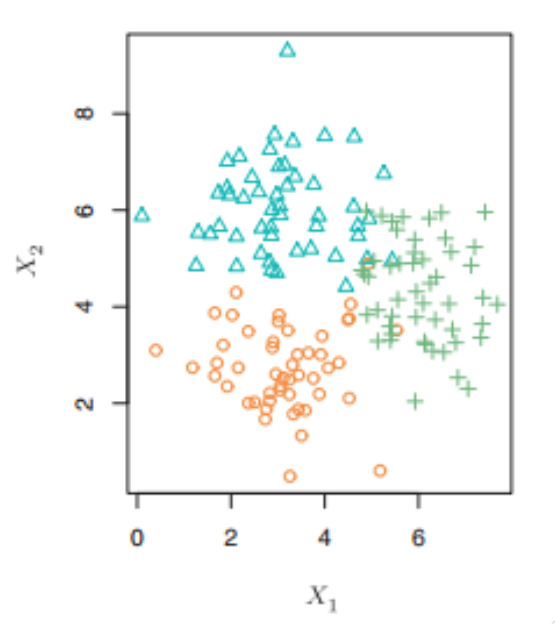
\includegraphics[scale=0.17]{unsupervised.png}
  \end{center}
\end{frame}
\begin{frame}[fragile=singleslide]
  \frametitle{Aprendizaje Supervisado y Terminología}
  \begin{itemize}
    \item Objetivo es predecir una variable, la \textit{etiqueta}. Puede ser de
      dos tipos:
      \begin{itemize}
        \item Si la variable es \textbf{categórica} (o discreta) se dice que el
          problema es de \textbf{clasificación} (binaria o multiclase)
          \begin{itemize}
            \item Construir un filtro de correo basura con mensajes anotados
              como \textit{spam/no-spam}
          \end{itemize}
        \item Si la variable es \textbf{continua} se dice que el
          problema es de \textbf{regresión}
          \begin{itemize}
            \item Predecir cantidad de ventas de un call center un día
              determinado
          \end{itemize}
      \end{itemize}
    \item ¿Cómo aprendemos? Seamos levemente más formales...
      \begin{itemize}
        \item Dado un vector de entrada $X$ y un vector de salida $Y$
          asumimos que existe una función (desconocida) tal que $f: X \to Y$:
          \begin{equation*}
            Y = f(X) +  \varepsilon
          \end{equation*}
          \begin{itemize}
            \item Aquí $f$ representa la información \textit{sistemática} que
              $X$ provee de $Y$ mientras que $\varepsilon$ es el \textit{error
              irreducible}.
          \item la literatura de ML llama \textit{target} a la variable
            explicada y \textit{features o atributos} a las explicativas.
          \end{itemize}
        \item Para encontrar (una aproximación) de $f$, \textbf{aprendemos por
          ejemplos}:
          \begin{enumerate}
            \item Construimos un \textbf{conjunto de entrenamiento} compuesto
              por $N$ ejemplos de la forma $\{\, (x_{1}, y_{1}), \ldots, (x_{N},
              y_{N}) \,\}$ donde $x_{i}$ e $y_{i}$ son respectivamente un
              \textbf{vector de atributos} (o features) y su etiqueta asociada.
            \item Los valores de entrada $x_{i}$ alimentan algún
              \textit{algoritmo de aprendizaje} que produces resultado $\hat{y}
              = \hat{f}(x_{i})$
            \item El algoritmo de aprendizaje modifica $\hat{f}$ minimizando las
              diferencias entre los resultados originales y los propiamente
              generados: $y_{i} - \hat{f}(x_{i})$.
          \end{enumerate}
      \end{itemize}
  \end{itemize}
\end{frame}
\begin{frame}[fragile=singleslide]
  \frametitle{Tipos de modelos}
  \begin{itemize}
    \item \textbf{Paramétricos}: asumen que $f$ toma una determinada forma
      funcional y utilizan el conjunto de entrenamiento para estimar los
      parámetros de dicha caracterización.
      \begin{itemize}
        \item Ejemplos: \enquote{modelo lineal},  $f(X) = \beta_{0} +
          \sum_{i=1}^{k}\beta_{i}{X}_{i}$ (otros: LASSO, GAM, etc.)
        \item Ventajas:
      \begin{itemize}
        \item más fáciles de estimar ya que se reduce a estimar un
          conjunto de paramétros (por ejemplo con mínimos cuadrados ordinarios)
        \item más fáciles interpretar (hacer inferencia)
      \end{itemize}
        \item Desventajas: al ser más rígidos no son tan buenos para hacer
          predicciones
      \end{itemize}
    \item \textbf{No Paramétricos}: no hacen supuestos sobre la forma funcional de $f$
      \begin{itemize}
        \item Ejemplos: árboles de decisión (bagging, boosting), vecinos más
          cercanos, SVM, etc.
        \item Ventajas: mejores para hacer predicciones
        \item Desventajas: más costosos de ajustar y difíciles de interpretar
      \end{itemize}
  \end{itemize}

  \textbf{¿Los modelos más flexibles son siempre mejores para predecir?}
\end{frame}
\begin{frame}[fragile=singleslide]
  \frametitle{Overfitting y Underfitting}
  \begin{center}
    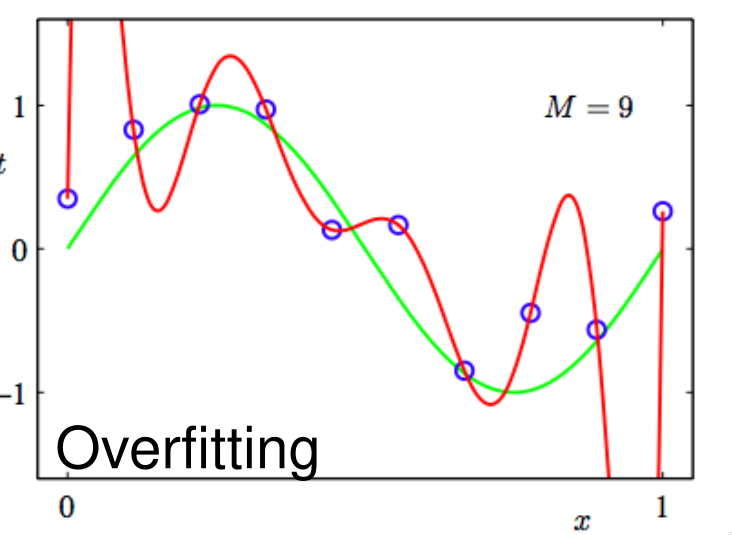
\includegraphics[scale=0.12]{overfitting.png}
    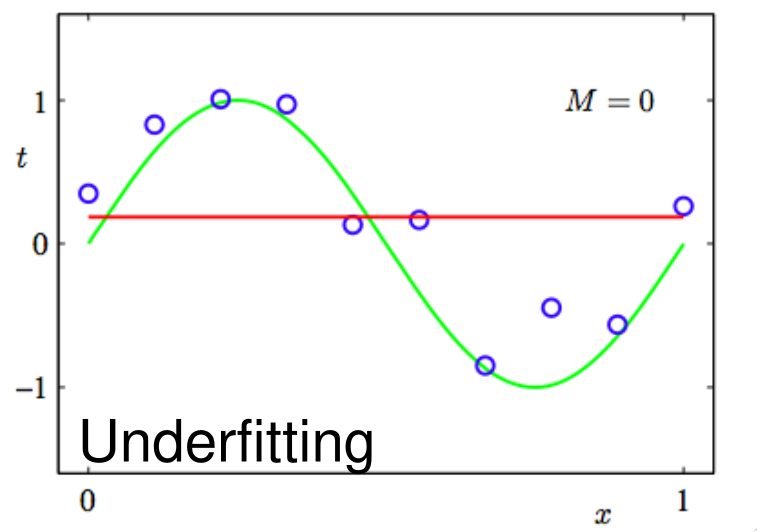
\includegraphics[scale=0.12]{underfitting.png}
  \end{center}
      % Dar ejemplo de colesterol por ejemplo
    \textbf{Objetivo final: obtener buenas predicciones en datos no observados previamente}
      \begin{itemize}
        \item La mayoría de los algoritmos ajusta utilizando observaciones
          $(x_{i}, y_{i})$ del conjunto de entrenamiento pero la performance es
          evaluada con observaciones y etiquetas de un \textit{conjunto de test}!
      \begin{itemize}
            \item \textbf{Overfitting}: el modelo se ajusta en exceso a la data
              de entrenamiento y no generalizá adecuadamente a datos nuevos
              \begin{itemize}
                \item Propia de modelos más flexibles que memorizan el
                  \enquote{ruido} y no propiedades verdaderas de la función a
                  estimar
              \end{itemize}
            \item \textbf{Underfitting}: el modelo es demasiado rígido y no
              captura relevantes con la consecuente mala performance en
              entrenamiento y test.
        \end{itemize}
    \item Algunas preguntas pendientes:
      \begin{itemize}
    \item ¿Qué forma funcional tiene una métrica de performance?
    \item ¿Es fácil obtener data de test?
    \item ¿Por qué ocurre el fenómeno de overfitting?
      \end{itemize}
  \end{itemize}
\end{frame}
\begin{frame}[fragile=singleslide]
  \frametitle{Selección de modelos: Conjunto de Validación}
  \begin{itemize}
    \item Repitamos nuevamente el objetivo de todo esto... \textbf{queremos predecir bien
      sobre datos desconocidos!}
    \item ¿Cómo hacerlo? Simulamos la división entre datos conocidos y
      desconocidos
          \begin{itemize}
            \item \textit{Enfoque de validation/holdout set}: entrenamos el
              modelo con datos conocidos y validamos las predicciones con el
              \textbf{conjunto de validación} (\enquote{desconocido})
              \begin{itemize}
                \item El conjunto de validación es una submuestra al azar de
                  observaciones del conjunto de entrenamiento (usualmente
                  20\%)
                \item Problemas: i) predicción de performance tiene alta
                  variabilidad ya que depende de la participación de
                  observaciones en entrenamiento/validación y ii) al achicar el
                  conjunto de entrenamiento podemos estar sobrestimando el error
                  de test
              \end{itemize}
           \end{itemize}
  \end{itemize}
  \begin{center}
    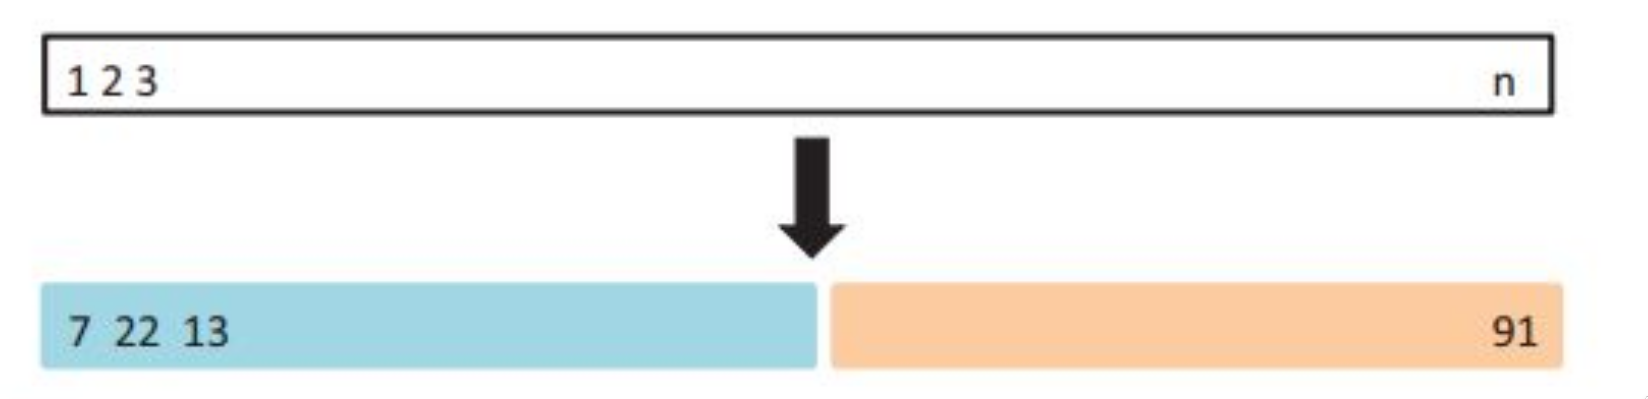
\includegraphics[scale=0.16]{holdout.png}
  \end{center}
  \textbf{¿Definido el modelo final: qué observaciones usamos para entrenarlo?}
\end{frame}

\section{Modelos de clasificación en Python}
\label{sec:modelos_de_clasificacion_en_python}

\begin{frame}[fragile=singleslide]
  \frametitle{Sin Datos No Hay Paraíso}
  \begin{center}
    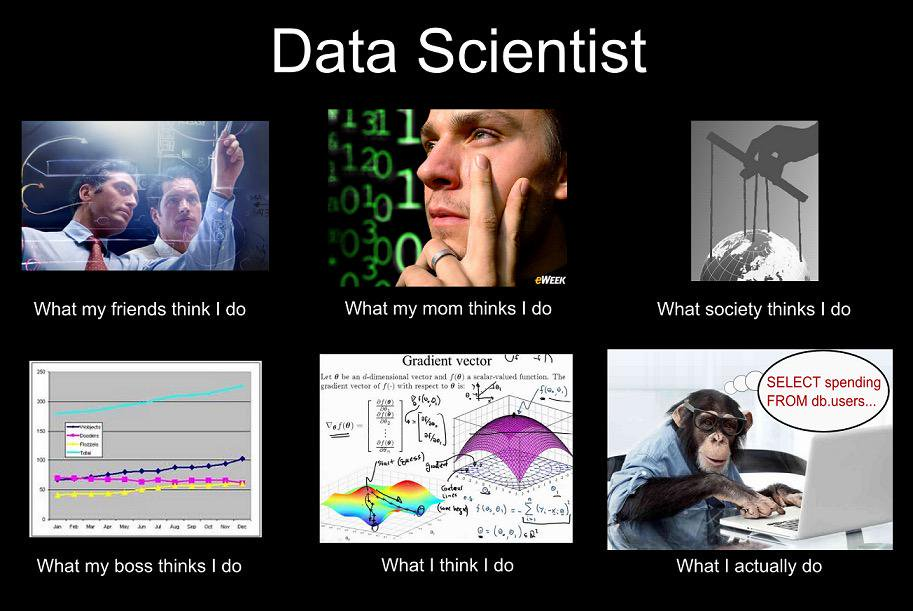
\includegraphics[scale=0.35]{whatido.jpg}
  \end{center}
\end{frame}
\begin{frame}[fragile=singleslide]
  \frametitle{Extracción de datos para clasificación}
  \begin{center}
    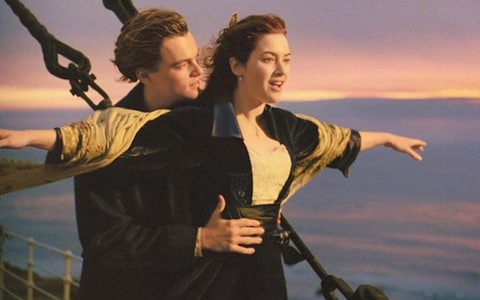
\includegraphics[scale=0.33]{titanic.jpg}
  \end{center}
  \begin{itemize}
    \item Objetivo: predecir (un subconjunto) sobrevivientes del Titanic (usando machine
      learning). Necesitamos datos!
      \begin{enumerate}
            \item \textit{Ejercicio 1: extracción de datos del hundimiento del Titanic}
              \begin{enumerate}
                \item Escriba una función que obtenga, a partir de
                  \href{http://biostat.mc.vanderbilt.edu/wiki/pub/Main/DataSets/titanic3.csv}{http://biostat.mc.vanderbilt.edu/wiki/pub/Main/DataSets/titanic3.csv} y utilizando Pandas, el conjunto de datos de pasajeros
                  involucrados en el hundimiento del Titanic y lo guarde en un
                  un archivo \texttt{titanic_local.csv}.$^{\dag}$
                \item Agregue lógica de cache que reuse la copia local del
                  conjunto de datos, en caso que esta exista, y evite de ese
                  modo consultar repetidas veces el enlace de arriba.$^{\dag}$
                \item Renombre la columna `home.dest` a `home\_dest`.$^{\dag}$
                \item Parta este conjunto de datos de forma aleatoria en dos
                  partes de manera tal que un subconjunto tenga el 70\% de los
                  registros.
                \item ¿Cómo puede garantizar que lo hecho en el inciso anterior
                  sea replicable?  Fije la semilla del generador de números
                  aleatorios en \texttt{1234.}
              \end{enumerate}
        \end{enumerate}
  \end{itemize}
\end{frame}
\begin{frame}[fragile=singleslide]
  \frametitle{EDA y ETFL}
  \begin{itemize}
    \item EDA: Análisis exploratorio de datos  (\textcite{tukey77})
      \begin{itemize}
        \item Data mining en su acepción pura: técnicas para analizar
          los datos, encontrar patrones y generar insights
          \begin{itemize}
            \item Visualizaciones: univariadas (para un mismo feature),
              bi-variadas (entre features y target), multivariadas (entre
              distintos features)
            \item Técnicas de estadística clásica: correlaciones, test de
              hipótesis, ANOVA
            % Analisis de componenetes principales (Pearson)
              % componentes ortogonales ordenados por variabiliad explicada
            \item Reducción de dimensionalidad: PCA, SVD
            \item Clustering
          \end{itemize}
        \item Objetivos:
          \begin{itemize}
            \item Comprender el dataset
            \item Definir y refinar la selección e ingeniera de atributos que
              alimentan los modelos
          \end{itemize}
      \end{itemize}
  \end{itemize}

  \begin{itemize}
    \item ¿Que es realmente hacer data science en la industria?
      \begin{itemize}
        \item \textbf{E}xtract \textbf{T}ransform \textbf{F}it \textbf{L}oad
        \item Distribución de tiempos: E 30\% T 50\% F 10\%, L 10\%
      \end{itemize}
  \end{itemize}
\end{frame}
\begin{frame}[fragile=singleslide]
  \frametitle{EDA e Ingeniería de atributos}
  \begin{itemize}
    \item El aprendizaje del algoritmo de aprendizaje dependerá de los
      atributos
      \begin{itemize}
        \item \textit{Garbage in - garbage out}
      \end{itemize}
      \item Técnicas diversas para generar/modificar atributos
        \begin{itemize}
          \item Transformaciones logaritmicas
            \begin{itemize}
              \item Tiene sentido cuando variables siguen una distribución
                asimétrica positiva (masa concentrada en valores pequeños y
                grandes con poca densidad)
            \end{itemize}
          \item Reescalamiento de variables numéricas
            \begin{itemize}
              \item Si el modelo es sensible a la escala del atributo es
                deseable hacer transformaciones tipo \textit{estandarización}
              \item Propenso a hacer \textbf{data leakage}: incorporar en los
                modelos información que no debería estar disponible al momento
                de puesta en producción
            \end{itemize}
          \item Binning
            \begin{itemize}
              \item Agrupación en \textit{bins} ordenados
            \end{itemize}
          \item Transformación de variables categóricas en variables continuas
            (\textit{one-hot encoding})
      \end{itemize}
  \end{itemize}
  \begin{center}
    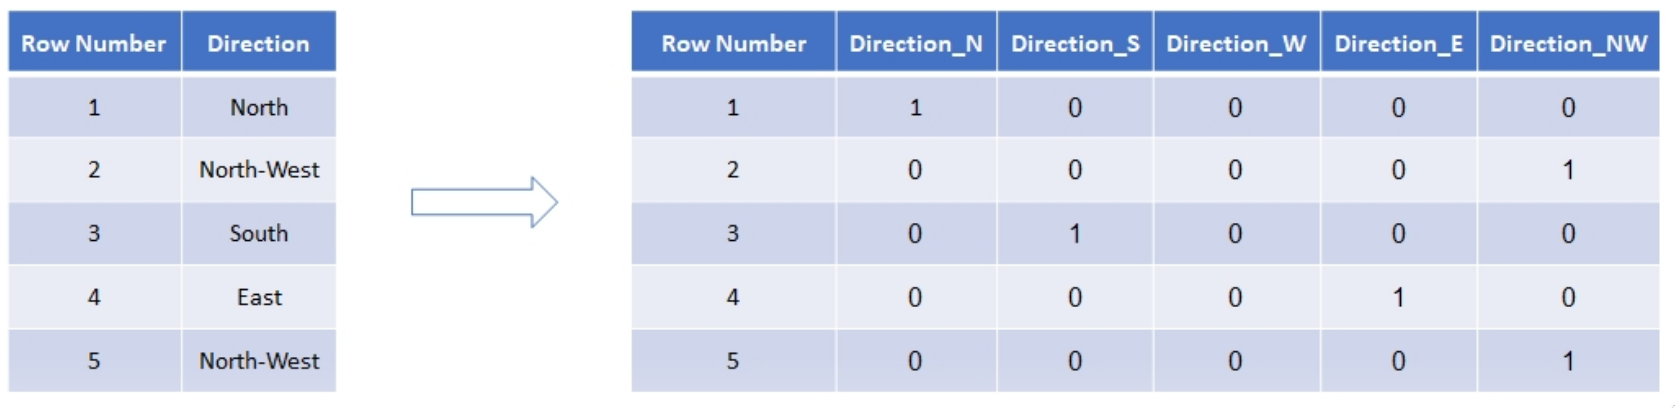
\includegraphics[scale=0.17]{one_hot.png}
  \end{center}
\end{frame}
\begin{frame}[fragile=singleslide]
  \frametitle{Descripción de variables y preprocesamiento}
  \begin{center}
    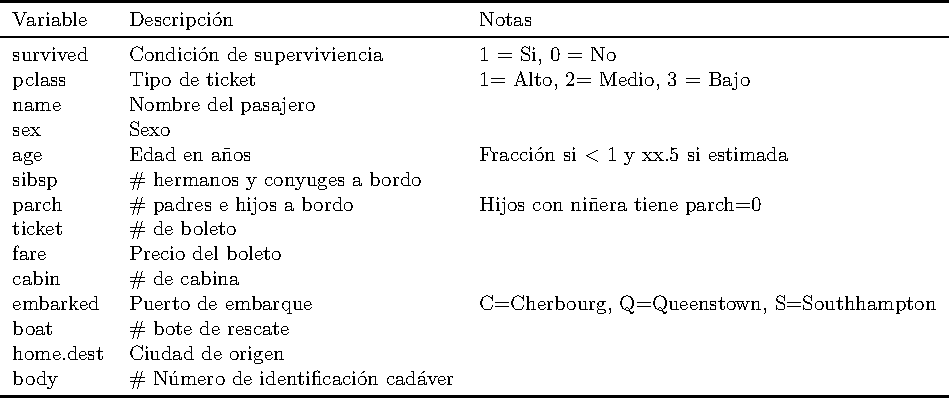
\includegraphics[scale=0.6]{table_variables.pdf}
  \end{center}
  \begin{itemize}
    \item En base a esta tabla:
      \begin{itemize}
        \item \textit{Ejercicio 2: Primer preproceso / EDA}
          \begin{enumerate}
            \item Escriba una función que permita convertir (\textit{castear})
              múltiples columnas de un tipo de dato a otro y utilícela para
              asegurar que sus datos sean consistentes con la tabla arriba.$^{\dag}$
            \item ¿Qué variables puede usted ignorar? ¿Por qué? Escriba una
              función que reciba un dataframe y una lista de columnas
              a eliminar y devuelva un el data frame sin estas columnas.
              Logguee cuáles columnas fueron eliminadas.$^{\dag}$
            \item Una los conjuntos de entrenamiento y validación en único
              dataframe con una columna de booleanos indicando pertenencia al
              conjunto de entrenamiento. ¿Por qué tiene sentido trabajar con un
              set de datos de esta forma?
            \item ¿Tiene clases desbalanceadas? Haga un gráfico de barras para
              responder esta pregunta.
          \end{enumerate}
      \end{itemize}
  \end{itemize}
\end{frame}
\begin{frame}[fragile=singleslide]
  \frametitle{Un poco más de EDA}
  \begin{itemize}
    \item Vamos a utilizar \texttt{Seaborn} para hacer algunas visualizaciones
      estadísticas.
      \begin{itemize}
        \item Veamos primero correlaciones de los atributos numéricos
        \begin{minted}{python}
        import seaborn as sns
        g = sns.heatmap(df.select('survived', 'age', 'parch', 'fare', 'sibsp')
                        .toPandas().corr(), annot=True, fmt = ".2f", cmap = "coolwarm")
        \end{minted}
        \begin{center}
          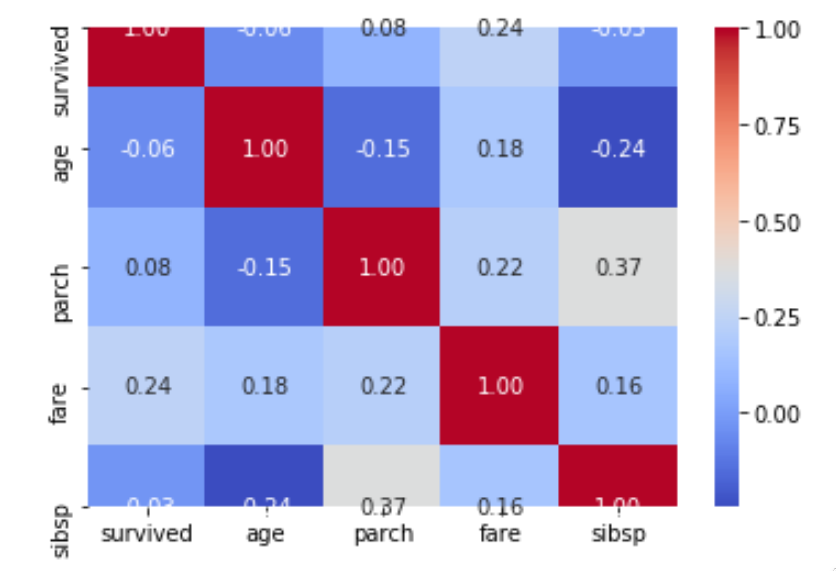
\includegraphics[scale=0.15]{corr.png}
        \end{center}
        \begin{itemize}
          \item Solamente el precio del boleto parece estar correlacionado con
            la probabilidad de supervivencia... ¿debemos descartar las otras
            variables?
        \begin{minted}{python}
        g = sns.FacetGrid(df, col='survived')
        g = g.map(sns.distplot, 'age')
        \end{minted}
        \begin{center}
          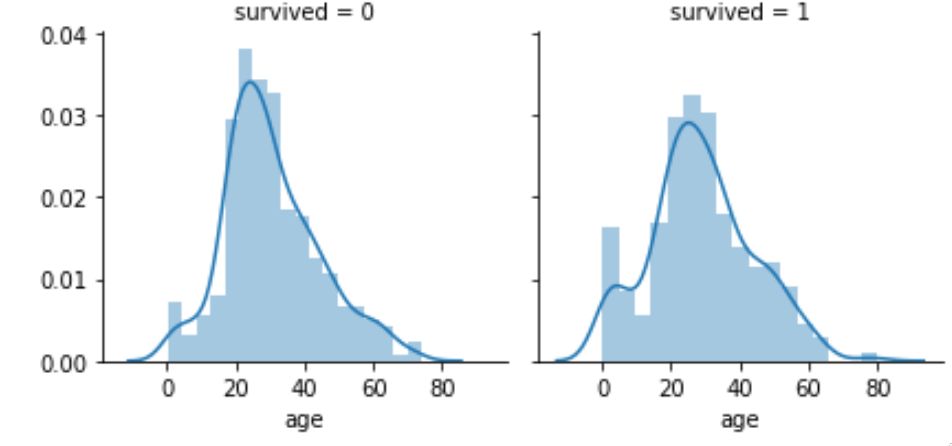
\includegraphics[scale=0.14]{facet.png}
        \end{center}
        \end{itemize}
      \end{itemize}
  \end{itemize}
\end{frame}
\begin{frame}[fragile=singleslide]
  \frametitle{Aun más EDA (y ejercicios)}
    \begin{minted}{python}
    survived_age = df.filter((f.col('survived') == 1) &
                   (f.col('age').isNotNull())).select('age').toPandas()
    ...
    g = sns.kdeplot(not_survived_age.squeeze(), color='Red', shade=True)
    g = sns.kdeplot(survived_age.squeeze(), color='Blue', shade=True)
    g.set_xlabel('age')
    g.set_ylabel('Frequency')
    g.legend(['Not Survived', 'Survived'])
    \end{minted}
    \begin{center}
      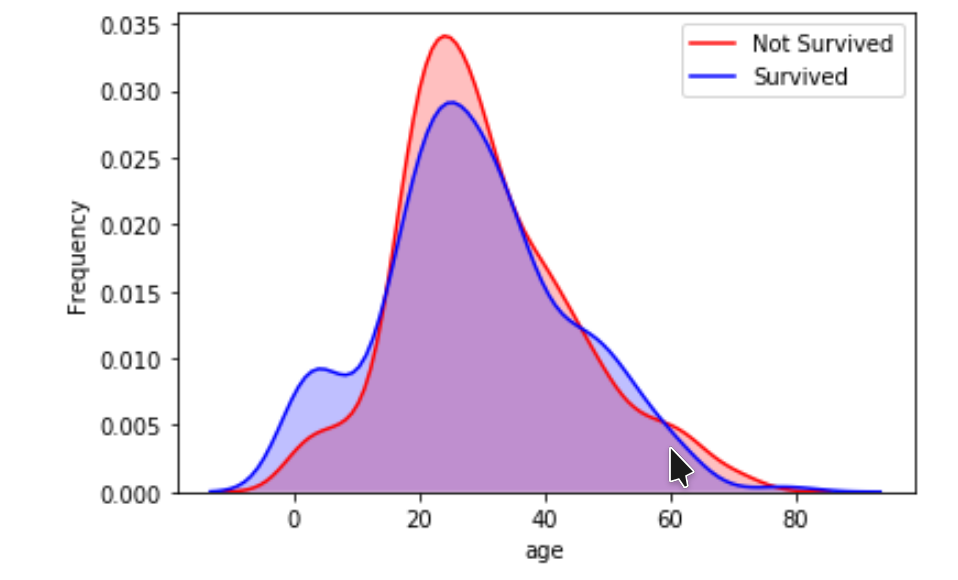
\includegraphics[scale=0.12]{kde.png}
    \end{center}
  \begin{itemize}
    \item \textit{Ejercicio 3: Visualizaciones como herramienta de EDA}
      \begin{enumerate}
        \item Use la función \texttt{distplot} para graficar la distribución del
          precio de boletos.
          \begin{enumerate}
            \item ¿Es la distribución resultante asimétrica/sesgada? En caso
              afirmativo aplique alguna transformación sobre la variable y
              grafique la nueva distribución.
          \end{enumerate}
        \item ¿Son los hombres o las mujeres más propensos a sobrevivir?
          Grafique la probabilidad de supervivencia para cada caso y compute el
          valor exacto de las mismas.$^{\dag}$
        \item ¿Hay alguna clase del barco que garantice mayor probabilidad de
          supervivencia? ¿Es este resultado robusto a controlar por sexo?
          \textit{Hint}: use la función \texttt{catplot}.
      \end{enumerate}
  \end{itemize}
\end{frame}
\begin{frame}[fragile=singleslide]
  \frametitle{Transformación (análisis univariado)}
  \begin{itemize}
    \item Valores faltantes, repetidos, constantes y extremos
    \begin{itemize}
        \item  ¿Cuál es la frecuencia de valores
          nulos o faltantes? ¿Vale la pena descartar por esto motivo alguna
          variable? ¿Imputamos valores? ¿Qué valor usar?
        \item ¿Tienen contenido informativo aquellas variable con nula o
          cuasi-nula varianza?
        \item ¿Tiene sentido reemplazar valores extremos?
  \end{itemize}
  \item \textit{Ejercicio 4: Trabajando con valores nulos y constantes}
    \begin{enumerate}
      \item Escriba una función que i) para cada atributo compute la proporción de
        valores nulos y ii) en caso que esta supere un determinado umbral
        elimine dicha columna
        \begin{enumerate}
          \item Potencialmente podría borrar información importantes (como el
            target!). ¿Cómo puede modificar la función anterior para proteger a
            esta columnas?
        \end{enumerate}
      \item En espíritu similar al punto anterior escriba una función que elimine,
        si las hay, columnas con nula o
        cuasi nula varianza.$^{\dag}$
      \item Escriba una función o lógica que permita rellenar valores de
        atributos numéricos por su mediana. ¿Cómo puede extender esto a
        atributos categóricos? % rellenar embark por ejemplo con mas frecuente
        \begin{itemize}
          \item Hint: le puede primero servir escribir una función auxiliar que
            identifique las columnas por tipo (categórica o numérica)
        \end{itemize}
      \item Sugiera/piense mejoras sobre el procesamiento hecho en los puntos
        anteriores. % edad podria ser primero correlacionada con tipo de ticket
        % y llenar de forma acorde (ejemplo los de 1era clase son mas viejos que
        % los de segunda)
    \end{enumerate}
  \end{itemize}
\end{frame}
\begin{frame}[fragile=singleslide]
  \frametitle{Ingenieria de atributos}
  \begin{quote}
    Applied Machine Learning is basically Feature Engineering (Andrew Ng)
  \end{quote}

    \begin{itemize}
      \item Hay muchas opciones para hacer ingeniería de atributos (por ejemplo
        extraer el título del nombre)
      \begin{itemize}
        \item \textit{Ejercicio 5: Ingeniería de atributos}
          \begin{enumerate}
            \item Cree un nuevo atributo \texttt{family_size} con el tamaño de
              la familia de cada pasajero (incluyendo a el mismo).$^{\dag}$
                \item Dado este nuevo atributo genere 3 atributos adicionales
                  que remitan a familias de un único miembro, de 2 a 4 miembros
                  y mayor o igual a 5.$^{\dag}$
                \item Haga uno (o varios) gráficos comparando la probabilidad de
                  supervivencia de cada una de estas familias.
              \item Bonus: Extraiga un prefijo a partir de la columna de boletos
                siempre y cuando el valor de esa columna no sea numerico.
                Reemplace esta columna por dicho prefijo.
          \end{enumerate}
      \end{itemize}
    \end{itemize}
\end{frame}
\begin{frame}[fragile=singleslide]
  \frametitle{Clasificación versus Regresión}
\begin{itemize}
  \item En general los conceptos del universo de problemas de regresión se
    trasladan al caso de clasificación con pequeñas diferencias
    \begin{itemize}
      \item Nuestro \textit{target} es ahora una variable discreta o
        categórica de forma que el objetivo es clasificar etiquetas
        desconocidas en distintas clases
      \item Numerosos problemas pueden modelarse de este modo
        \begin{itemize}
          \item Rotulado de correo basura, churn, probabilidad de default, etc
        \end{itemize}
      \item Queremos que nuestro clasificador estimado, $\hat{f}$, minimice
        ahora la siguiente función
      \begin{equation*}
        \frac{1}{p}\sum_{i=1}^{p}I(y_{i} \not = \hat{y}_{i})
      \end{equation*}
      donde $I(\cdot)$ es una función que vale 1 si $y_{i} \not = \hat{y}_{i}$
        y 0 en caso contrario.
        \begin{itemize}
          \item Básicamente deseamos reducir la proporción de errores que
            cometemos
        \end{itemize}
      \item Esencialmente estamos intentando buscar una frontera de decisión
        óptima (en el sentido que minimice el error de arriba)
        \begin{itemize}
          \item Algunos \enquote{clasificadores} conocidos: Bayes ingenuo,
            k-vecinos más cercanos, regresión logística, etc
        \end{itemize}
    \end{itemize}
\end{itemize}
\begin{center}
  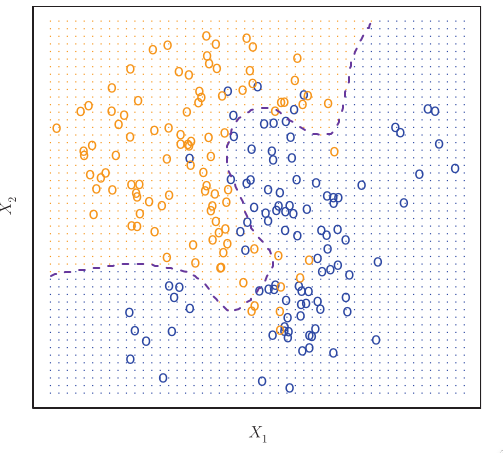
\includegraphics[scale=0.15]{frontier}
\end{center}
\end{frame}
\begin{frame}[fragile=singleslide]
  \frametitle{Regresión Logística}
  \begin{itemize}
    \item Supongamos que queremos modelar la probabilidad que un cliente cancele
      o no su línea de celular
    \begin{itemize}
      \item Podriamos pensar en un modelo de regresión lineal como los ya
        vistos:
        \begin{equation*}
          Y_{t} = \beta_{0} + \beta_{1}X_{t-k} + \varepsilon_{t}
        \end{equation*}
        \begin{itemize}
          \item En base a esto definir un cliente \enquote{cancelador} si $\hat{Y} > 0.5$
          \item Pero ... el target no caerá necesariamente en el intervalo $[0,1]$.
        \end{itemize}
      \item Tiene sentido en cambio formular el problema como
      \begin{equation*}
        \Pr(Y_{t} = 1) = F(\beta_{0} + \beta_{1}X_{t-k} + \varepsilon_{t})
      \end{equation*}
      donde $F(\cdot)$ es la función logística dada por $F(\cdot) = \frac{1}{1 + e^{-x}}$
    \end{itemize}
  \end{itemize}
    \begin{minted}{python}
    >>> x = np.linspace(-5, 5, 100)
    >>> y = 1 / (1 + np.exp(-x))
    >>> plt.plot(x, y)
    \end{minted}
    \begin{center}
      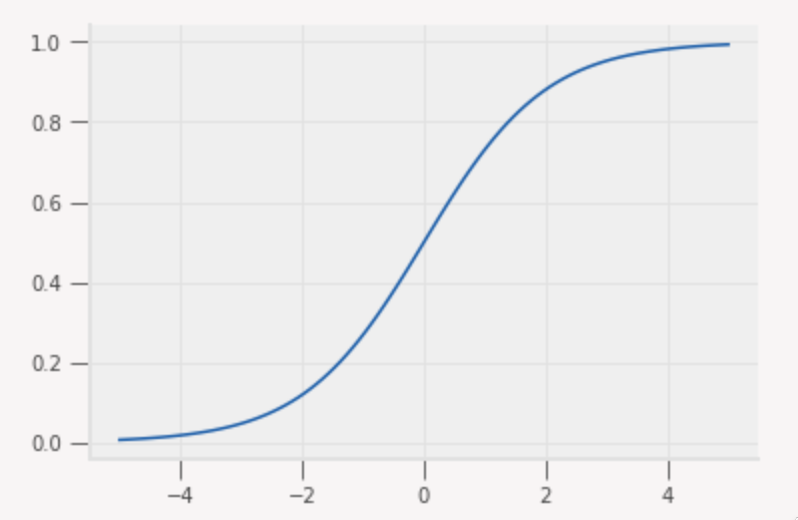
\includegraphics[scale=0.15]{logistic.png}
    \end{center}
\end{frame}
\begin{frame}[fragile=singleslide]
  \frametitle{Métricas de performance}
  \begin{itemize}
    \item En general estos modelos devuelven estimaciones de
      \textit{probabilidades condicionales}. ¿Cómo sabemos si fueron buenas?
    \begin{itemize}
      \item Necesitamos alguna métrica de evaluación. Una \textbf{matriz de
        confusión} nos permite definir algunas
        \begin{center}
          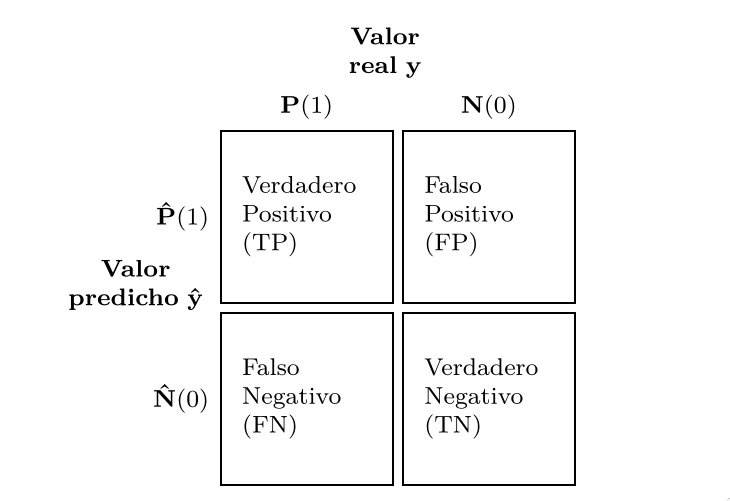
\includegraphics[scale=0.2]{confusion_matrix.png}
        \end{center}
        \item Hay dos tipos de errores: \textbf{falsos positivos}
          y \textbf{falsos negativos}
          \begin{itemize}
            \item Podemos derivar métricas en base a estos errores
            \item La más \enquote{natural} se conoce como exactitud o
              \textbf{accuracy} definida por el ratio de clasificaciones
              correctas sobre el total realizado:
              \begin{equation*}
                \frac{TP + TN}{TP + TN + FP + FN}
              \end{equation*}
            \item ¿Es una buena métrica? Puede ser engañosas...
          \end{itemize}
    \end{itemize}
  \end{itemize}
\end{frame}
\begin{frame}[fragile=singleslide]
  \frametitle{Clases Desbalanceadas}
  \begin{center}
    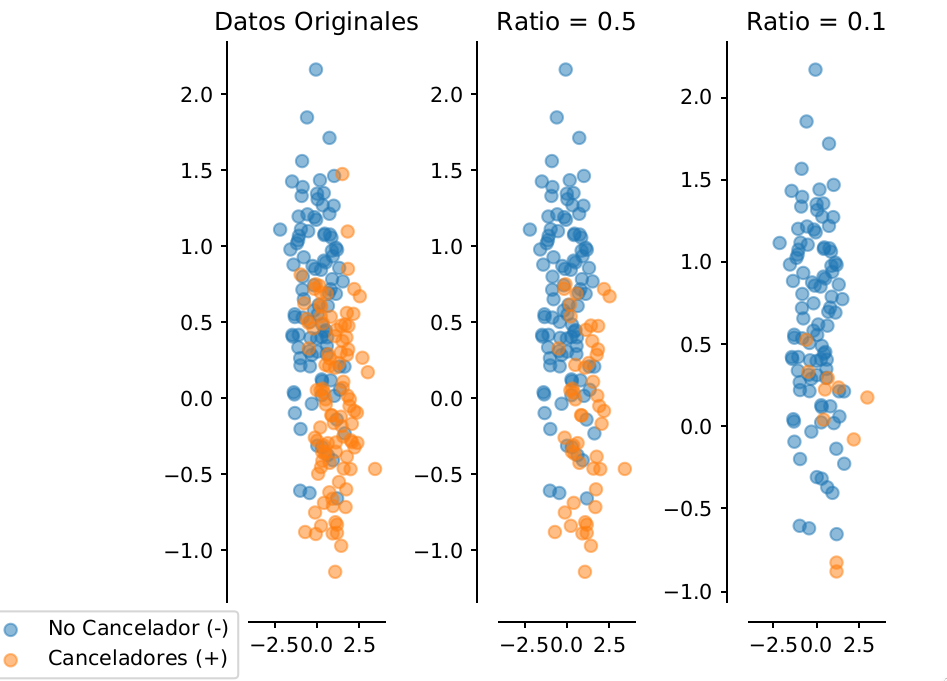
\includegraphics[scale=0.2]{unbalance_class.png}
  \end{center}
  \begin{itemize}
    \item Imaginemos el caso último panel con una proporción de 1 caso
      positivo cada 100
      \begin{itemize}
        \item Un clasificador trivial que prediga siempre la clase negativa
          tiene una exactitud del 99\%.
        \item ¿Podemos construir una métrica para evitar esta situación? Hay
          que tratar de evitar mezclar los verdaderos positivos y negativos...
      \end{itemize}
  \end{itemize}
\end{frame}
\begin{frame}[fragile=singleslide]
  \frametitle{Precisión, cobertura y F1 Score}
  \begin{itemize}
    \item Para sortear los problemas anteriores es frecuente utilizar las
      siguiente dos métricas
      \begin{itemize}
        \item \textbf{Precisión}: cantidad de casos correctamente rotulados
          como positivos sobre el total de predicciones positivas, $TP / (TP +
          FP)$.
        \item \textbf{Cobertura o Recall}: proporción de instancias positivas
          que el algoritmo logra identificar sobre el total de casos positivos
          ($TP / (TP + FN)$)
        \item Depende del contexto puede ser deseable maximizar una o la otra
          \begin{itemize}
            \item Si es una enfermerdad rara, por caso, nos interesa más la
              cobertura que la precisión. ¿Para un filtro de spam?
          \end{itemize}
      \end{itemize}
      \begin{itemize}
        \item En determinadas situaciones ambos métricas son importantes y
          tiene sentido combinarlas
          \begin{equation*}
            F_{1} = 2\frac{p\cdot r}{p + r}
          \end{equation*}
          \begin{itemize}
            \item Pesa por igual a ambas métricas (media harmónica) y el
              valor suele estar cerca del mínimo de las métrica
            \item Esta acotado al intervalo $[0, 1]$ y vale 1 únicamente para
              un clasificador perfecto
            \item Valores superiores a 0.7 son propios de un \enquote{buen}
              clasificador
            \item Desventaja: no hace un juicio sobre como el modelo clasifica
              las instancias negativas
          \end{itemize}
      \end{itemize}
  \end{itemize}
\end{frame}
\begin{frame}[fragile=singleslide]
  \frametitle{La curva ROC}
  \begin{center}
    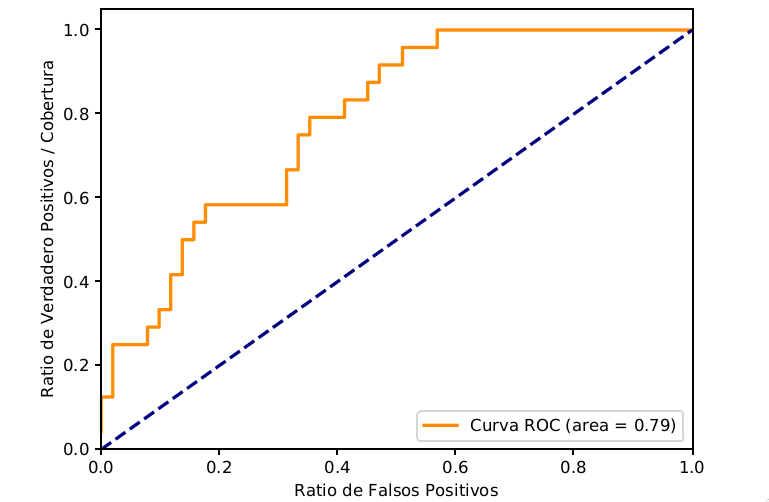
\includegraphics[scale=0.2]{roc.png}
  \end{center}
  \begin{itemize}
    \item Características:
      \begin{itemize}
        \item Para definir pertenencia a una clase hay un umbral, $p$, tal que
          si $p=0$ (1) siempre (nunca) predigo que las observaciones son
          positivas entonces ambos TPR (TP / P) y FPR (FP/ N) valen 1 (0)..
        \item Curva 45 grados define a un clasificador aleatorio y la
          coordenada $(0,1)$ a un clasificador perfecto
        \item Intuitivamente si elegimos aleatoriamente una observacion
          positiva y una negativa el area bajo la curva es la probabilidad de
          que el clasificador rankee más alto al positivo
      \end{itemize}
  \end{itemize}

  \textbf{Conviene utilizar una única métrica para guiar las decisiones}
\end{frame}
\begin{frame}[fragile=singleslide]
  \frametitle{Fitteo del modelo}
  \begin{itemize}
    \item Estamos casi listos para predecir sobrevivientes usando una regresión
      logística
      \begin{itemize}
        \item \textit{Ejercicio 6: Fit Regresión Logística}
          \begin{enumerate}
            \item Alguno algoritmos, en Python, soportan exclusivamente
              atributos numéricos.
              Escriba entonces una función que utilice \textit{StringIndexer} para
              convertir todos los atributos categóricos.\\
              Bonus: ¿Tiene sentido usar esta codificación para
                atributos que carecen de orden? En caso contrario pruebe
                emplear \textit{One-Hot-Encoding}.
            \item Fitee una regresión logística sobre la data de entrenamiento y
              genere predicciones (y probabilidades) para la data de test/validación.
            \item Evalue estas predicciones usando métricas
              de \textit{accuracy} y ROC para el conjunto de entrenamiento y ROC
              para el conjunto de validación.$^{\dag}$
            \item Bonus: utilice \texttt{scikit-learn} o escriba una función
              que compute la métrica \texttt{F1} y con ello evalué nuevamente
              los resultados para ambos conjuntos.
          \end{enumerate}
      \end{itemize}
  \end{itemize}
\end{frame}
\begin{frame}[fragile=singleslide]
  \frametitle{Sobre train, validation, test split}
  \begin{itemize}
    \item ¿Podemos overfittear el conjunto de validación?
      \begin{itemize}
        \item Si realizamos muchas pruebas posiblemente si
        \item Por eso en la práctica trabajamos con 3 conjuntos:
          entrenamiento, validación y testeo
        \begin{center}
          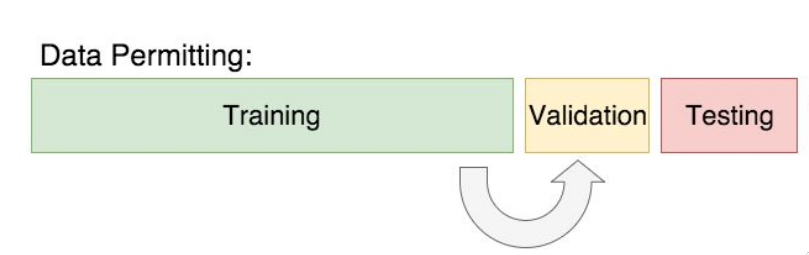
\includegraphics[scale=0.3]{tvt.png}
        \end{center}
        \begin{itemize}
          \item En general se reserva 20\% para testing y el remanente se
            divide en 80\% entrenamiento y 20\% validación
          \item Con muchos datos los porcentajes son menores: es una cuestión
            de representatividad y no de números
          \nocite{james13}\nocite{efron16}
        \end{itemize}
      \end{itemize}
  \end{itemize}
  \begin{center}
    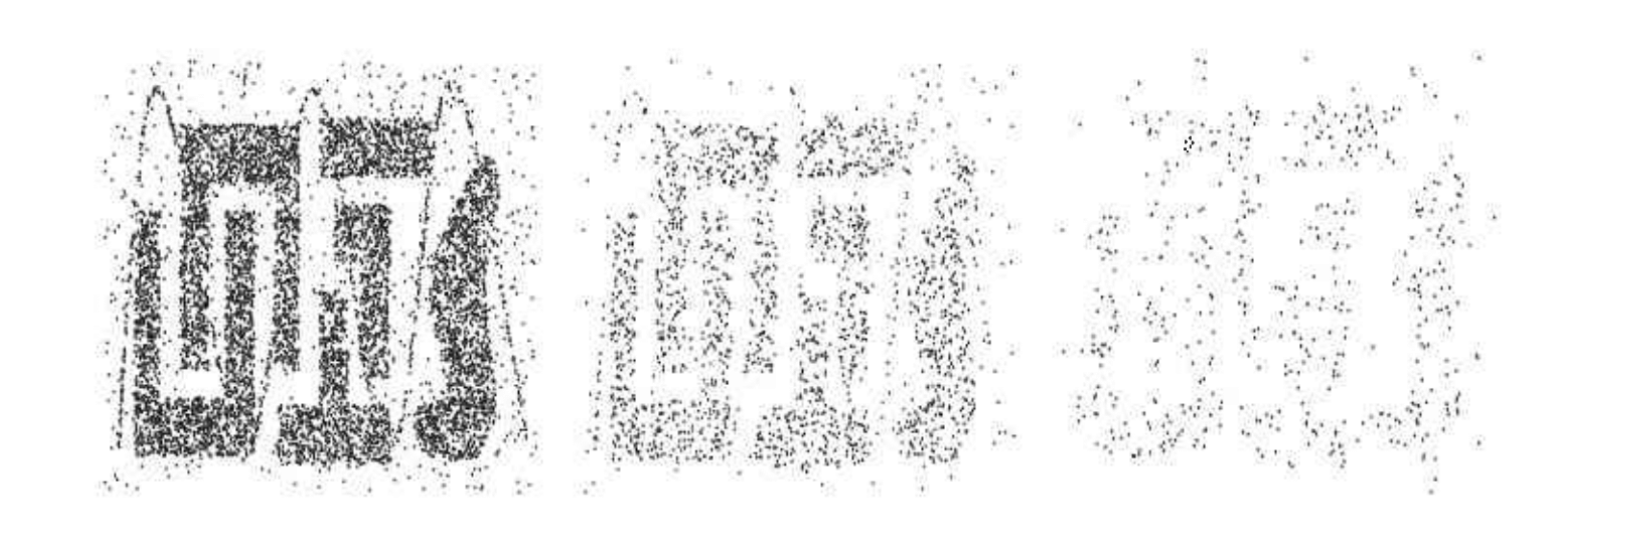
\includegraphics[scale=0.32]{sample_size.png}
  \end{center}
\end{frame}
\begin{frame}[fragile=singleslide]
  \frametitle{Tradeoff de Sesgo-Varianza}
  \begin{itemize}
    \item ¿Cuál es el valor esperado de ECM en una observación de testeo?
      \begin{itemize}
        \item Es decir cuál es el ECM promedio si uno estima sucesivas veces
          $f$ usando muchos conjuntos de entrenamiento y evaluando en cada $x_{0}$
            del conjunto de test:
      \begin{equation*}
        E(y_{0} - \hat{f}(x_{0}))^{2} = \var(\hat{f}(x_{0})) +
        \left[Sesgo(\hat{f}(x_{0}))\right]^{2} + \var(\varepsilon)
      \end{equation*}
      donde
      \begin{itemize}
        \item La varianza remite a cuánto cambiaría $\hat{f}$ si estimaramos
          con otro conjunto de entrenamiento (idealmente queremos que sea
          poco)
        \item El sesgo alude a si $\hat{f}$ está errando consistentemente en
          las predicciones ($Sesgo(\hat{f}(x_{0})) = E[\hat{f}(x_{0})] -
          y_{0}$).
        \item El ideal: tener un sesgo bajo y una varianza baja. ¿Es esto
          posible?
      \end{itemize}
  \end{itemize}
  \end{itemize}
  \begin{center}
    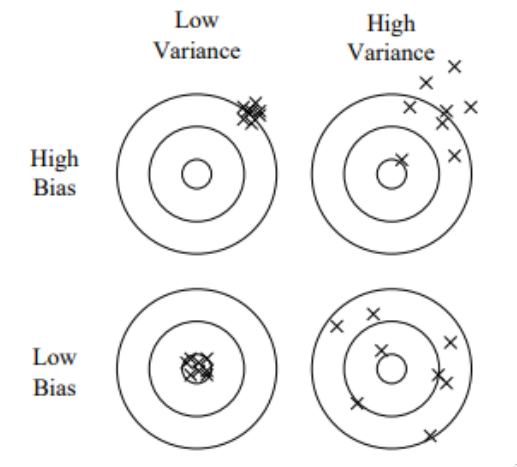
\includegraphics[scale=0.2]{bias_variance_tradeoff.png}
  \end{center}
\end{frame}
\begin{frame}[fragile=singleslide]
  \frametitle{Tradeoff Sesgo-Varianza II}
  \begin{center}
    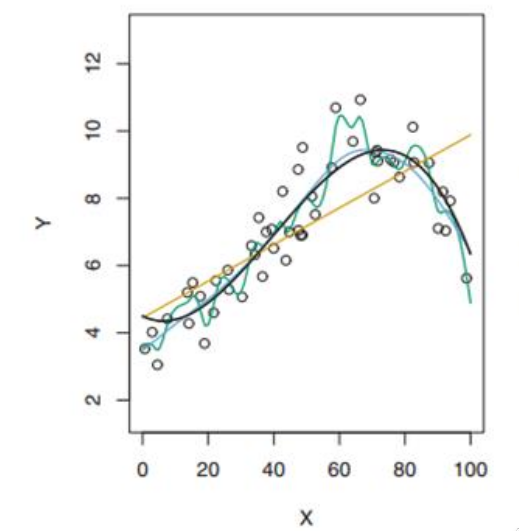
\includegraphics[scale=0.25]{bvt2.png}
    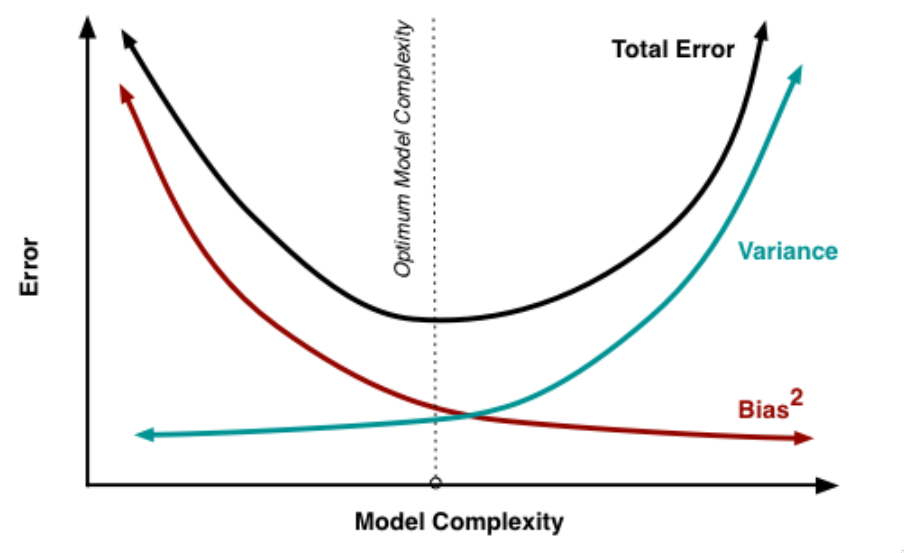
\includegraphics[scale=0.225]{complexity.png}
  \end{center}
  \begin{itemize}
    \item ¿Por qué hay un tradeoff?
      \begin{itemize}
        \item Es fácil obtener un método con bajo sesgo y alta varianza
          (dibujando una curva que pase por todos los puntos)
        \item Es fácil obtener un método con bajo o nula varianza y alto sesgo
          (fitteando una constante)
      \end{itemize}
    \item En general vale lo siguiente
      \begin{itemize}
        \item Métodos más complejos tienen alta varianza y bajo sesgo
        \item El fenómeno de \textit{overfitting} se asocia a escenarios
          justamente de alta varianza y bajo sesgo
      \end{itemize}
  \end{itemize}
\end{frame}

\section{Árboles y ensamble de modelos}
\label{sec:arboles_y_modelos_de_}

\begin{frame}[fragile=singleslide]
  \frametitle{Árboles de decisión}
  \begin{itemize}
    \item Característica central: particionan el espacio de atributos en
      regiones
      \begin{itemize}
        \item Cada región está definida por el cumplimiento de alguna regla
        \item Particionar de esta manera define una \textbf{estructura de árbol}
          (con nodos terminales o hojas, nodos internos y ramas (aristas))
          por el cumplimiento de alguna regla
          \begin{center}
            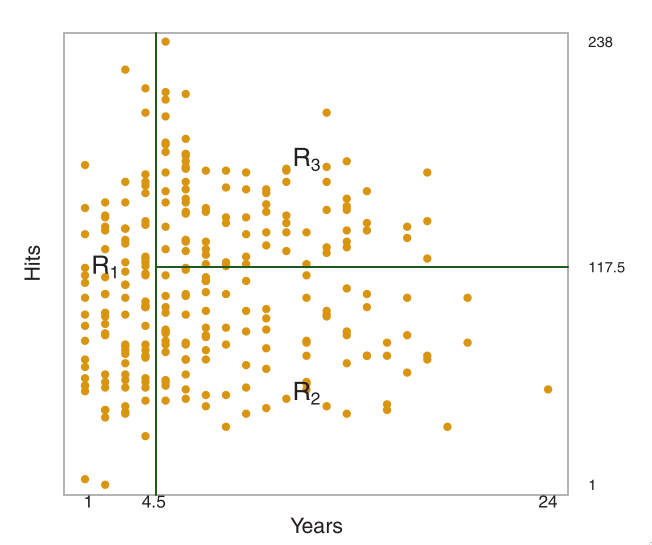
\includegraphics[scale=0.2]{tree_regions.png}
            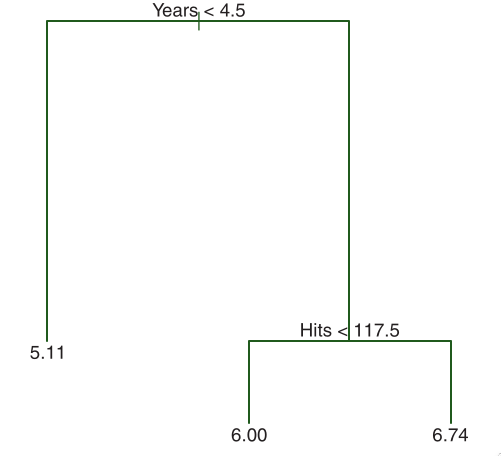
\includegraphics[scale=0.23]{tree.png}
          \end{center}
      \end{itemize}
    \item ¿Cómo podemos utilizar esto para problemas de clasificación?
      \begin{itemize}
        \item Una observación dentro de una determinada región pertenecerá a la
          clase más frecuente en esa región: ¿cómo elegimos las regiones?
      \end{itemize}
  \end{itemize}
\end{frame}
\begin{frame}[fragile=singleslide]
  \frametitle{Particionamiento recursivo binario}
  \begin{itemize}
    \item Proceso iterativo que funciona del siguiente modo
      \begin{enumerate}
        \item Se fija un criterio para hacer cortes
          \begin{itemize}
            \item En clasificación resulta natural
usar el \textit{error de clasificación} de cada región: para una región $m$ con $N_{m}$ observaciones la proporción de observaciones
que no pertenecen a la clase $k$ resulta ser
\begin{equation*}
  EC = \frac{1}{N_{m}}\sum_{i\in R_{m}}I(y_{i} \not = k)
\end{equation*}
          \end{itemize}
      \item Para el primer nodo seleccionamos el predictor y el punto de corte
        tal que particionar el espacio de atributos en dos regiones, genere la
          mayor reducción en el error de clasificación.
      \item Para los nodos de decisión
siguientes repetimos el proceso en cada (sub)región resultante hasta llegar a algún criterio de parada
      \end{enumerate}
  \item Ventajas:
    \begin{itemize}
      \item Fáciles de interpretar si no son muy profundos
      \item Excelente manejo de no linealidades
      \item Sencillo obtener un resumen de la importancia de cada atributo
    \end{itemize}
  \item Desventajas:
    \begin{itemize}
      \item  Poco sesgo (decreciente en profundidad) pero altisima varianza (basta considerar partir el
        conjunto de entrenamiento de forma aleatoria en mitades)
    \end{itemize}
  \end{itemize}
\end{frame}
\begin{frame}[fragile=singleslide]
  \frametitle{Bagging y Árboles aleatorios}
  \begin{itemize}
    \item Bagging:
      \begin{itemize}
        \item En general vale que agregar observaciones reduce la varianza
          \begin{itemize}
            \item Podemos crear $B$ conjuntos de entrenamiento muestreando de forma
              aleatoria (y con reposición) del conjunto entrenamiento original
              (\textit{bootstraping}).
              \end{itemize}
            \item Si luego entrenamos sobre cada conjunto y promediamos
              reducimos la varianza (y tenemos bajo sesgo)
              \begin{equation*}
                \hat{f}_{bag}(x) = \frac{1}{B}\sum_{b=1}^{B}\hat{f}^{*b}(x)
              \end{equation*}
            \item La predicción final es la clase más votada por los $B$
              árboles (regla mayoritaria)
      \end{itemize}
    \item Random Forests: ideado por Breiman con el objeto de mejorar
      aun más la performance predictiva
      \begin{enumerate}
        \item Al igual que en bagging se crean $B$ conjuntos de entrenamiento muestreando de forma
          aleatoria (y con reposición) del conjunto entrenamiento original.
        \item Para cada conjunto se hacer particionamiento recursivo pero al
          elegir los cortes se emplea un subconjunto aleatorio de la totalidad
          de atributos (\textit{descorrelacionar})
      \end{enumerate}
  \end{itemize}
\end{frame}
\begin{frame}[fragile=singleslide]
  \frametitle{Ejercicios Árboles}
  \begin{itemize}
    \item \textit{Ejercicio 7: Árboles de decisión y aleatorios}
      \begin{enumerate}
        \item Fittee un árbol de decisión en vez de una regresión logística y
          compare la performance de los modelos.$^{\dag}$
          \begin{itemize}
            \item Bonus: Grafique el árbol de decision resultante
          \end{itemize}
        \item Repita el punto anterior pero ahora con un bosque
          aleatorio.$^{\dag}$
          \begin{itemize}
            \item Bonus: Pruebe aumentar la profundidad del árbol. ¿Mejora su métrica de
                    performance?
          \end{itemize}
        \item Compute y grafique la importancia de atributos.
      \end{enumerate}
      \begin{center}
        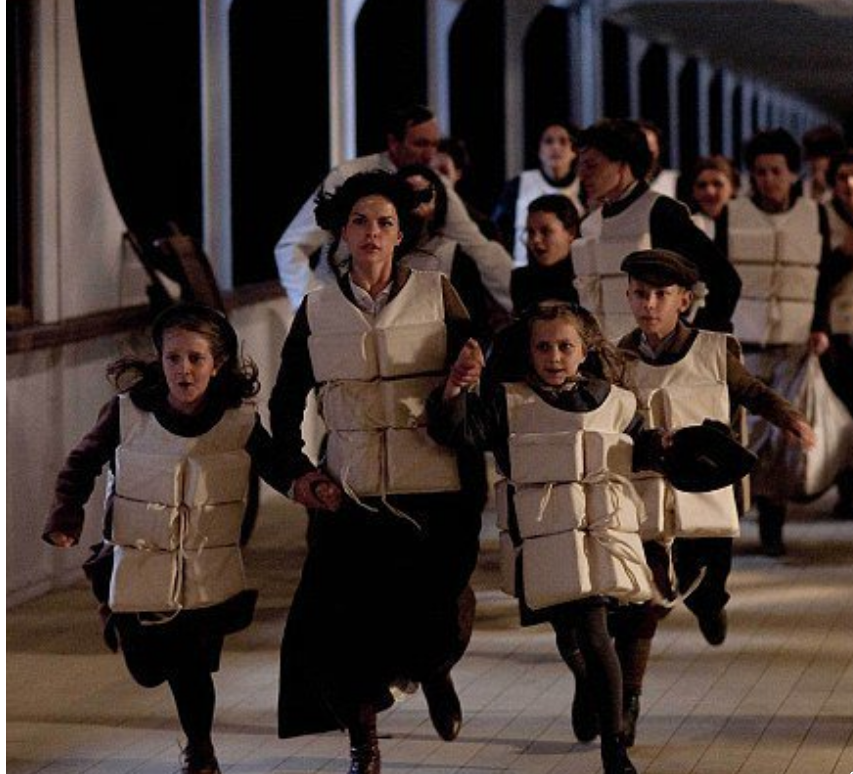
\includegraphics[scale=0.18]{run.png}
      \end{center}
  \end{itemize}

\end{frame}

\section{Conclusión}
\label{sec:aprendizaje_no_supervisado}
\begin{frame}[fragile=singleslide]
  \frametitle{Comentarios finales}
  \begin{itemize}
    \item Tenemos una mejor idea de data science y en particular machine
      learning con Python y Spark.
    \item Sin embargo... hay muchas cosas que (obviamente) no vimos
    \begin{itemize}
      \item No vimos aprendizaje no supervisado ni reinforcement learning
      \item ... ni tampoco un ejemplo de regresión
      \item Prácticamente no hemos trabajado con datos fechados!
        \begin{itemize}
          \item El mecanismo de train/test split debe tener una noción
            temporal
        \end{itemize}
        \item Hay otros métodos de selección de atributos
          \begin{itemize}
            \item Arboles no profundos y hacer feature importance para
              identificar features o Lasso sobre regresión.
          \end{itemize}
          \item Técnicas de reducción de dimensionalidad
          \item Técnicas de corrección de desbalance e clases
          \item Tuneo de hiperparámetros
    \end{itemize}
  \end{itemize}
\end{frame}



\begin{frame}[fragile=singleslide]
  \frametitle{Referencias}
  \begin{columns}
    \column{0.85\paperwidth}
    \printbibliography
  \end{columns}
\end{frame}
\end{document}
